\section{Implementation}
\label{sec:implementation}
  \subsection{Neural Network Algorithm Implementation}
  
\begin{frame}
  \centering
  \begin{figure}
    \only<1-3>{
        \begin{subfigure}[b]{0.3\textwidth}
          \caption{Free Positioning}
                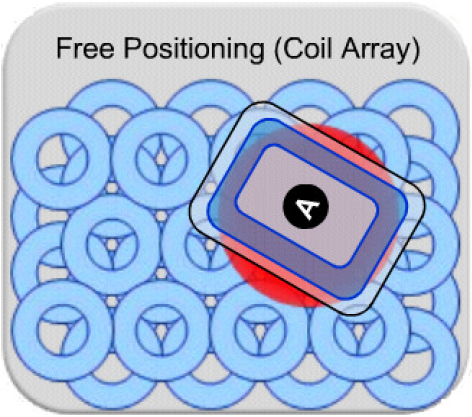
\includegraphics[width=\textwidth,height=\textwidth]{./png/multiple}
                \label{fig:guided}
                \setcounter{subfigure}{0}% Reset subfigure counter
        \end{subfigure}\hfill
        }
    \only<2-3>{
        ~ %add desired spacing between images, e. g. ~, \quad, \qquad etc.
          %(or a blank line to force the subfigure onto a new line)
        \begin{subfigure}[b]{0.3\textwidth}
        \setcounter{subfigure}{1}% Reset subfigure counter
          \caption{Neural Network}
                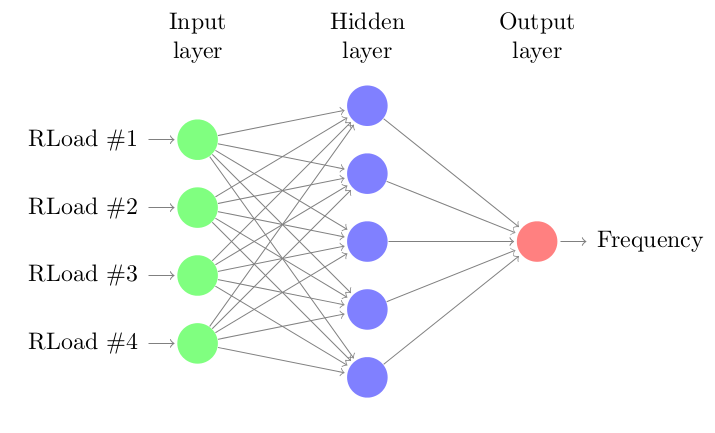
\includegraphics[width=\textwidth,height=\textwidth]{./png/neural}
                \label{fig:free}
        \setcounter{subfigure}{0}% Reset subfigure counter
        \end{subfigure}\hfill
        }
    \only<3-3>{
        ~ %add desired spacing between images, e. g. ~, \quad, \qquad etc.
          %(or a blank line to force the subfigure onto a new line)
        \begin{subfigure}[b]{0.3\textwidth}
            \setcounter{subfigure}{2}% Reset subfigure counter
          \caption{Matlab Output}
                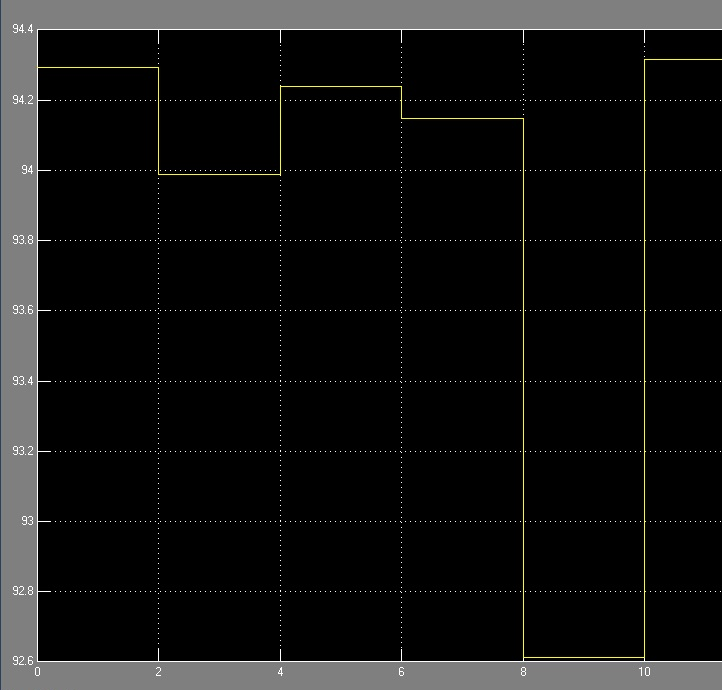
\includegraphics[width=\textwidth,height=\textwidth]{./png/output}
                \label{fig:multiple}
        \end{subfigure}%
        }
        \caption{Different wireless charging approaches~\label{fig:animals}~\cite{wsn}}
  \end{figure}
  \begin{itemize}[<+->]
      \item<1-| alert@1>> Free positioning charging based on Inductive coupling~\cite{wireless}.
      \item<2-| alert@2>> Based on RLoad and Frequency Input and Output ~\cite{wireless}. %\ref{fig:free}
      \item<3-| alert@3>> Simulation of Matlab Output based on RLoad as an Input~\cite{wireless}. %\ref{fig:multiple}
    \end{itemize} 
\end{frame}
